\documentclass[12pt]{cutecv}
\usepackage[english]{babel}
\usepackage{hyperref}
\usepackage{graphicx}

\newcommand{\listbullet}{$\; \cdot \;$}

\author{Ксения Сырбулова}
\contacts{tg: @naysudes | +79639699628 | syrbulova@gmail.com}
\begin{document}

\maketitle

\columnratio{0.3,0.7}
\begin{paracol}{2}
\setlength{\columnsep}{2em}
\setlength{\cvsectionverticalskip}{5mm}
\setlength{\cvinfoverticalskip}{5mm}

\begin{leftcolumn}
  \vspace{5mm}
  \begin{figure}[htp]
    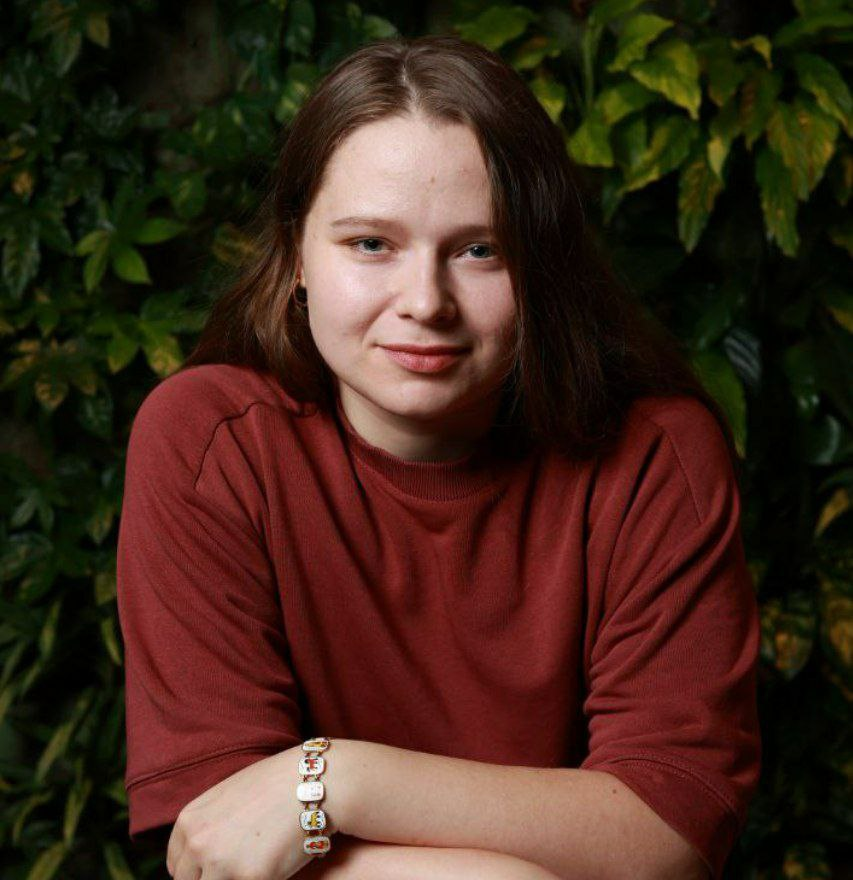
\includegraphics[width=5cm, height=5cm]{image.jpg}
\end{figure}

\begin{cvsection}{Ключевые навыки}
  \listbullet Backend \listbullet User-space networking \listbullet Алгоритмы \listbullet Базы данных
   \listbullet Распределеленные системы \listbullet Concurrency
   \listbullet Производительность \\
\end{cvsection}

\begin{cvsection}{Языки программирования}
  Golang \listbullet Python \listbullet C++
\end{cvsection}

\begin{cvsection}{Технологии}
  Linux \listbullet Kafka \listbullet RabbitMQ
  gRPC \listbullet PostgreSQL \listbullet  MongoDB \listbullet Docker \listbullet Kubernetes
  \listbullet Git \\
\end{cvsection}

\end{leftcolumn}

\begin{rightcolumn}
\begin{cvsection}{Опыт работы (4 года)}
  \cvinfobox{Яндекс.Такси}{ 02.2022-по настоящее время | Python Разработчик}
  {Разрабатывала сервисы Биллинга Такси. Поддержка нового функционала (пайплайны выплат и взаимозачета), 
  оптимизировала обработку данных и добавляла вспомогательный функционал (сверки выгрузок данных и выплат). \\
  \underline{Технологии:} Python и C++ в качетсве языков, PostgreSQL и YDB в качестве баз данных. \\
  \underline{Достижения:} \\ \listbullet Проект моментыльных выплат для водителей, в ходе которого
  смогли сократить время ожидания выплат на карту водителей с суток до 5 минут. \\
  \listbullet Потоковые сверки выгрузок данных, благодаря которым был предотвращен финансовый инцидент на крупную сумму.}
  
  \cvinfobox{Прикладная логистика}{ 06.2020-02.2022 | С++ Разработчик}
  {Разрабатывала программу учета для заводских производств. Создавали понятный интерфейс
  и систему защищенную от падений и потери данных. \\
  \underline{Технологии:} C++ и PostgreSQL. Qml и QT в качетсве фреймворков для создания интерфейсов.\\
  \underline{Достижения:} Самостоятельно разработала модуль учета для модели грузовика и сдала его заказчикам без дополнительных правок.}
\end{cvsection}
\begin{cvsection}{Образование}
  \cvinfobox{МГТУ им. Н.Э. Баумана }{2016-2020 | Прикладная механика}{Диплом бакалавра}
  \cvinfobox{Технопарк Mail.ru | VK Образование}{2021-2022 | Системный архитектор}
    {Два года подготовки full-stack инженеров, с курсами по БД, фронтенду и бекеду, а так же SRE.}
  \cvinfobox{ШАД (Школа анализа данных)}{2023-2024 | Проектирование распределенных систем} {Углубленный курс по распеделенным системам, с погружением в сети, внутрнности БД и эксплуатацию сервисов. }
\end{cvsection}
\end{rightcolumn}
\end{paracol}

\end{document}
